\documentclass{article}

\usepackage{latexsym}
\usepackage[pdftex]{graphicx}
\usepackage{amsmath}
\usepackage[left=1in,top=1in,right=1in,nohead,nofoot]{geometry}

\pagestyle{empty}

\begin{document}

\title{Numerical Simulation of Planet Formation in the Solar System}
\author{John Boggs, Cameron Froehlich, Peter Reinhardt}
\maketitle

\begin{figure} 
 \begin{center}
 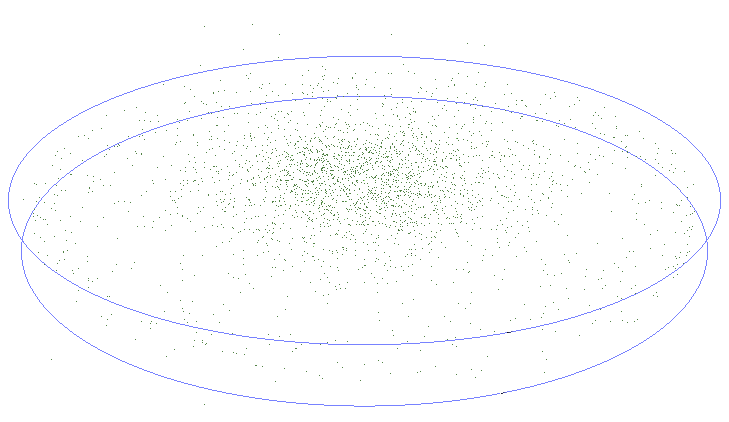
\includegraphics[scale=0.5]{screenshot.png} 
 \caption{Screen shot of the simulation after three integration steps.} 
 \end{center}
\end{figure}

\section{Abstract}
In this project, we simulated accretion in the early solar system. Massive particles are randomly dispersed in a cylindrical space surrounding a much larger mass. The masses and initial velocities are random gaussian variables, but the velocities tend to a particular orbital direction. The system is then numerically integrated using the Euler method, accounting for gravitational interactions between all the masses.

We will statistically analyze the mass, orbital characteristics, and the frequency of collisions. We will vary the existence of a large secondary body (i.e. Jupiter) and the mean and variance of the distributions of mass, initial velocities and initial positions.

\section{Resources and Applicability}
The only resources necessary to this project are several computers, a working C++ compiler and a copy of Matlab for data analysis. These resources are readily available.

The simulation involves kinematics and the physics of gravity and inelastic collisions. This is certainly in the realm of 8.012.

\section{Background}
The presently accepted model of the formation of our solar system is the nebular model. In the nebular model, the planets formed from a vast amount of rotating interstellar material, flattened into a disk along their rotational axis. Particle collisions, known as accretion, gradually increased the mass of the individual particles, and decreased the amount of particles in the system. This process eventually lead to the formation of planets.[7]

It is also believed that the formation of large gas giant planets occurs before the formation of small, inner planets. The gravitational perturbations created by the large secondary body disrupt the otherwise orderly rotation of the inner nebular disc, causing increased rates of accretion.[1][3]
	
N-body simulations are used to model accretion. The n-body simulation is a numerical approximation of the gravitational interactions of three or more particles in space. Using positions and velocities determined by the n-body simulation it can be determined whether or not particles will collide and accrete. Over time these collisions result in larger and larger bodies, eventually forming planets.[4]
\[\]\[\]

\section{Pseudocode}
initialize the particles' velocity, position and mass\\
create a particle at the origin with the mass of the sun\\
\noindent while (elapsed simulation time \verb <  end time) \{ \\
\indent for (each pair of particles) \{\\
\indent\indent if the particles have collided, combine them\\
\indent\indent increment the net acceleration with the gravitational acceleration between the two particles\\
\indent \}\\
\\
\indent for (each particle) \{\\
\indent\indent use the calculated accleration and timestep to update the position and velocity\\
\indent \}\\
\noindent\}\\

\section{Simulation Parameters}
\subsection{Constants}
The mass of the central body was assumed to be $m_S = 1.98892 \times 10^{30}$ kg, or one solar mass. The large secondary body was given the orbital characteristics and mass of Jupiter, $M_J = 317.8$ Earth masses. The total mass of the other simulated particles was approximately $100$ Earth masses, about the combined mass of the other major planets and the asteroid belt.[2][6]

\subsection{Distributions of Other Parameters}
The mass of the particles is given by a gaussian distribution with an average equal to the total non-solar mass in the solar system divided by the number of particles. The standard deviation of this distribution is $1\%$ of the average mass.

The position of the particles is given by a uniform distribution in cylindrical coordinates: radius, theta, and height.

The velocity of the particles is given by a gaussian distribution with an average equal to the velocity necessary to produce a circular orbit. The velocity out of the plane has a gaussian distribution with average zero and standard deviation $1\%$ of the average velocity.

\section{Physics}
\subsection{Gravity}
In order to find the net acceleration of each particle in the system, we calculate the gravitational acceleration due to each of the other masses in the system. For the $i^{th}$ particle of N total particles, the net acceleration is
\[\vec{a}_i(t) = \sum_{j=1, j\neq i}^{N} \frac{Gm_j}{||\vec{r}_{ij}(t)||^3} \vec{r}_{ij}(t)\]
Where $\vec{r}_{ij} = \vec{r}_i - \vec{r}_j$ is the vector between the $i^{th}$ and $j^{th}$ particles. To reduce simulation time, the gravitational force between two particles is only calculated once.

\subsection{Kinematics}
Using Euler's method of integration, the acceleration due to gravity can be used to predict the future position and velocity of the particles.
\[\vec{v}_i(t + \Delta t) = \vec{v}_i(t) + (\Delta t) \vec{a}_i(t)\]
\[\vec{r}_i(t + \Delta t) = \vec{r}_i(t) + (\Delta t) \vec{v}_i(t) + \frac{(\Delta t)^2}{2} \vec{a}_i(t)\]

\subsection{Collisions}
A fundamental problem in numerical many-body simulations of realistic masses is that collisions are extremely rare. In order to simulate a reasonable amount of time, the timestep must be reasonably large. With these large timesteps, the particles can pass through or right next to each other without the simulator finding a collision.

To avoid this, we use two methods for collision detection: the distance between the particles is less than the sum of the radii OR the relative velocity of the smaller mass is less than the escape velocity of the larger mass. Mathematically, the first condition is (ignoring constants close to unity):
\[||\vec{r}_i - \vec{r}_j|| \leq \sqrt[3]{\frac{m_i}{\rho}} + \sqrt[3]{\frac{m_j}{\rho}}\]
and the second condition is theoretically
\[||\vec{v}_i - \vec{v}_j|| \leq \sqrt{\frac{2Gm_i m_j}{min(m_i,m_j) ||\vec{r}_{ij}|| }}\]
To avoid long time-profile collisions between particles and the two major initial bodies (Jupiter and the Sun), only the first, radius-based method was used for collisions involving Jupiter or the Sun.

\section{Model Verification}
To verify that the numerical integration, units and graphics were all working, we used the Earth-Sun two particle system as a test. To do this we used a timestep of $\Delta t = 0.1$ days, a solar mass of $m_S = 1.98892 \times 10^{30}$ kg, an Earth mass $m_E = 5.9736 \times 10^{24}$ kg, initial Earth-sun distance $1$ AU $= 149598000$ km, and initial Earth velocity $v_E = 2573251.2$ km/day. Since each new frame is rendered after 100 steps, each frame corresponds to approximately $10$ days. The period of motion of the Earth about the center of mass is therefore expected to be about $36$ or $37$ frames. This is exactly what is observed (see video with filename `verification.avi').

\section{Results and Conclusions}
Although the model was greatly simplified to reduce simulation time, a week's worth of computation by a $2$ Ghz processor produced only 60 frames, or $1.2$ million steps of $0.1$ days each, for a total simulated time of $328.5$ years. The results can be seen in the movie titled `results.wmv'.

\subsection{Mass Distribution}
The mass distribution shows a flattening in the initial distribution and the creation of higher mass particles. This is expected in the accretion model, but the basic accretion idea does not conclusively suggest whether the accreted mass is distributed among a small number of larger bodies or a greater number of slightly less massive bodies. As can be seen in figure 2, the mass did not simply accrete into one super-mass, but instead accreted into numerous larger bodies. This lends some support to the relatively recent proposal that huge collisions were rampant in the early solar system. For example, it is now believed that the Moon was formed from the collision of the Earth and a Mars-sized body.[8] If our model is correct in predicting that many of these medium-sized bodies are created, huge collisions of the Moon-forming type would be frequent at later times.

\subsection{Particle Count}
The number of particles also decreases over time, apparently sub-linearly. We assume an exponential fit, which gives $particle\ count = 2980e^{-0.00015t}$ where $t$ is measured in years. If we extrapolate this fit into the future, the total number of bodies will dip below $100$ by $t = 23000$ years. This corresponds to an average mass per body of about one Earth mass. Most analyses done predict that the terrestrial planets form within $10-100$ million years.[5] Our estimate is significantly smaller than these other estimates because our starting particle size was relatively large (to make the simulation complete in a reasonable amount of time).

\subsection{Orbital Characteristics}
From figures 4 and 5 we can see that the largest planetoid created during the accretion process forms about $7.5$ AU from the Sun. This is just outside Jupiter's orbit at $5$ AU, suggesting that the third-largest body in the system is most likely to accrete just outside the orbit of the large secondary body. In fact, the orbit of Saturn is roughly $9.5$ AU. The results indicate that all the other planetoids form between $3$ AU and $12$ AU. For comparison, the orbit of Mars is $1.5$ AU and the orbit of Uranus is $20$ AU.

Figures 4 and 5 also show the creation of a trail of particles in highly elliptical or hyperbolic orbits. The trail lies roughly between $4$ and $10$ on the graph, which corresponds to orbits between $55$ AU and $22000$ AU. This corresponds roughly to the Oort cloud, a body of comets and other bodies on elliptical orbits lying within a $50000$ AU sphere.

\begin{figure} 
 \begin{center}
 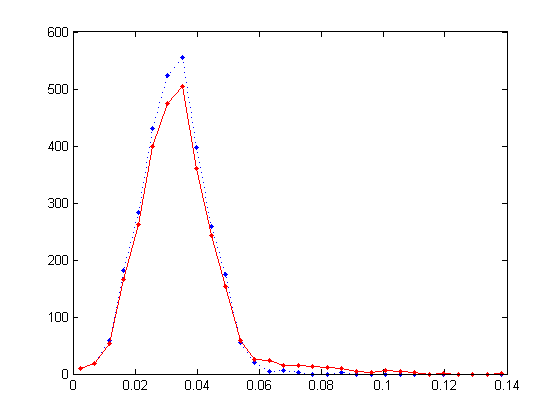
\includegraphics[scale=0.8]{massdistribution.png} 
 \caption{Distribution of mass initially (dotted) and finally (solid)}
 \end{center}
\end{figure}

\begin{figure} 
 \begin{center}
 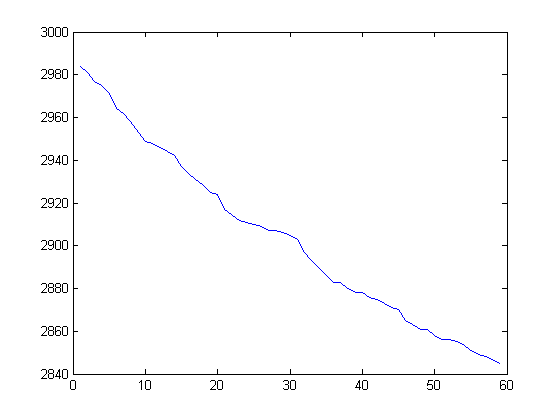
\includegraphics[scale=0.8]{particlecount.png} 
 \caption{Number of particles vs. time}
 \end{center}
\end{figure}

\begin{figure} 
 \begin{center}
 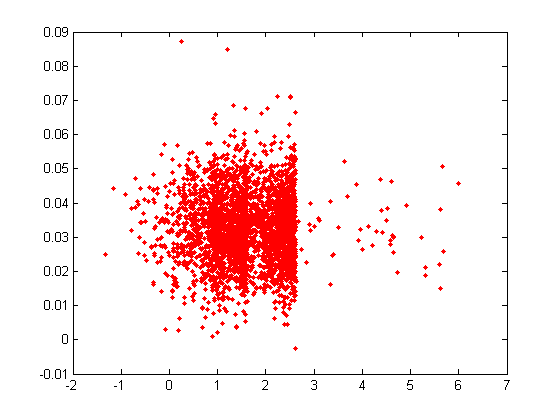
\includegraphics[scale=0.5]{massdistribution1.png} 
 \caption{Initial: particle mass (Earth masses) vs. log distance from sun (log(AU))}
 \end{center}
\end{figure}

\begin{figure} 
 \begin{center}
 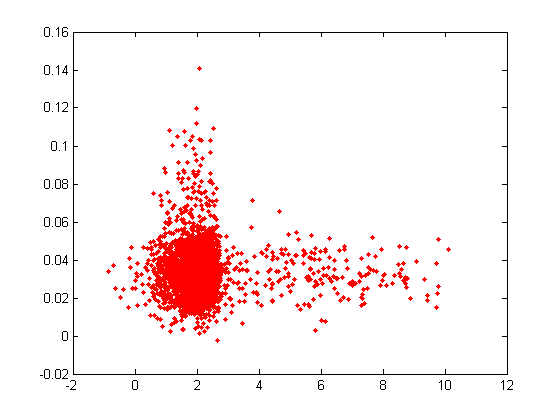
\includegraphics[scale=0.5]{massdistribution2.png} 
 \caption{Final: particle mass (Earth masses) vs. log distance from sun (log(AU))}
 \end{center}
\end{figure}

\end{document}